

\chapter{Preliminaries}\label{chapter:preliminaries}


\section{Containerization with Docker}

In recent years, container technology has gained widespread adoption in the software development world. By greatly simplifying the software deployment—and development workflow, containers have become a cornerstone of successful software architectures.
Considering their advantages over hypervisor-based virtualization, such near native performance, sub-second boot times \cite{felter2015updated}\cite{morabito2015hypervisors} and minimal disk space usage, containers bring qualities to the table that are relevant specifically to embedded systems.
Containers are independent units of deployment containing everything a particular application needs to run from system libraries, tools, and runtimes to application specific settings. 
Akin to hypervisor-based virtualization, Linux containers aim to provide isolated, self-contained execution environments for applications that may be moved freely between hosts without affecting the application’s behavior.

Unlike traditional virtual machines, however, applications in containers run on non-virtualized hardware, and thereby, with minimal performance overhead when properly configured \cite{felter2015updated}\cite{morabito2015hypervisors}. This is of interest particularly in the field of embedded systems where resource constraints are prevalent.
Enabled by the concept of \emph{kernel namespaces}, multiple containers may run on the same host at the same time without affecting one another, or even having knowledge of each others existence. 
Namespaces wrap a set of system resources and present them to the container process as if they were dedicated to it. Each aspect of a container runs in its own namespace and its access is limited to that namespace. Hence, a level of isolation is achieved that was previously only possible with virtual machines. The only thing containers share is the host’s OS kernel, and optionally, parts of the file system.

To which extent a container may use the host system's resources is controlled through a mechanism called \emph{cgroups}, which is shorthand for \emph{control gorups}. 
Cgroups is a Linux kernel feature that allows to limit the resources availabe to a group of processes. Containers, effectively being groups of processes, may therefore be alloted a certain amount of computing resources. This allows for fine-grained control over the resource utilization of individual containers running on a host system.

Docker \cite{DockerWebsite} is undoubtably the most prominent container technology and arguably the first one to make Linux containers accessible for general use. 

\subsection{Docker Images}
Unique to Docker is its approach to container images. Images may be seen as the ``blueprint'' on the basis of which containers are built. 
Images are implemented utilizing UnionFS, a Linux service that facilitates the layering of different file systems atop each other. 
Leveraging this technology, Docker images are made of layers, with each layer adding to, or modifying, the respective underlying layer. 
A benefit of this approach is that individual layers may be shared and reused in other containers, thereby saving tremendous amounts of disk space compared to traditional VM images.

\subsection{Docker Networking}



\section{Container networking with Weave Net}

Weave was choses because, to this date, it is the only solution that supports both, multicast and encryption. Competing tools are flannel and dockernet.


%\begin{figure}
%  \centering
%  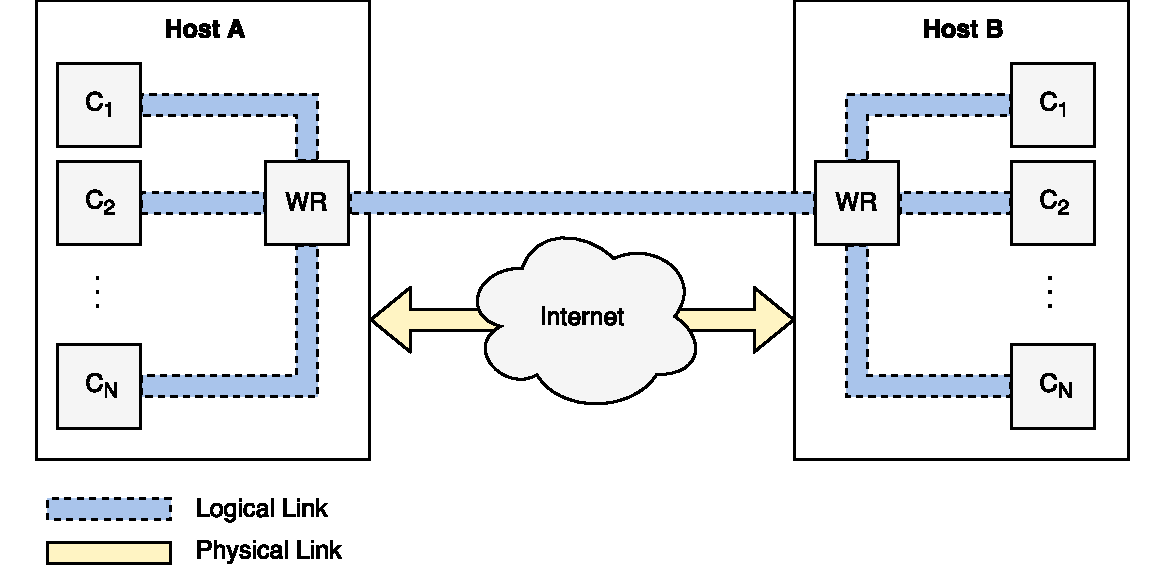
\includegraphics[width=\textwidth]{include/sdn.pdf}
%  \caption[SDN]{Connecting containers using Weave Net.}\label{fig:sdn}
%\end{figure}


\section{Continuous Integration}



\section{Communication}

What has been discussed so far is what services are and how they can be implemented. One question that remains is how they are connected. SOA, being a pattern for distributed systems, requires its components to communicate with each other over a network.

Which communication patterns are there?

push vs. pull,
unicast vs. multicast
synchronous vs. asynchronous
centralized vs. decentralized

What makes PubSub especially attractive?
PubSub enables loose coupling. No apriori knowledge of communication partners required. Hardware independence: Services may be migrated between computing nodes. Abstraction of underlying infrastructure is important.
No startup dependencies: The order in which services finish initializing is irrelevant. Especially important with ephemeral services.


\section{Data Distribution Service}

What is DDS?
DDS is a messaging middleware standard for distributed applications. 
The underlying principle of it is data centric publish-subscribe.
What does data centric mean?
Designed for mission- and business critical systems.
Offers transport transparency.
"virtual global data space": Each component views a data store like it is local but in actuality it is distributed.
data-centric instead of message-centric. The difference is that the former implies a shared data model. The middleware has an understanding of the data and its context and is responsible that all components have a common view of the data.
The advantage of data-centric messaging is that it allows a higher abstraction. Developers can focus on the data itself and on developing business logic instead of having to implement data sharing through exchange of messages.

DDS is a message bus. This is in contrast to a broker-based architecture. A broker enables flexible routing patterns featuring filtering, variable numbers of message queues etc. However, it can be considered a single point of failure.

Being a standard, DDS strives for interoperability between implementations

\paragraph{Dynamic Service Discovery}
Offers dynamic service discovery.


\paragraph{Quality of Service}
One of DDS's salient features is its intrinsic QoS support implemented by \emph{QoS policies}.
QoS policies specify service attributes for controlling each participant's behavior and quality properties. They can be set for each participant and topic individually. An example for a QoS policy is the \texttt{DEADLINE} policy. It specifies the minimum message frequency of a service. If the deadline period of a hypothetical data writer is set to, e.g., 100 ms, that means that this data writer is required to send a message at least every 100 ms. If it fails to send a message at this rate, the data writer and all the respective topic's readers will need to deal with this circumstance on a code level. 

In addition, QoS policies serve as service contracts. They specify non-functional requirements that services must fulfill to be able to communicate with each other. E.g., a service provider's \texttt{RELIABILITY} policy may have been set to the \texttt{BEST\_EFFORT} level, thereby allowing the service to drop samples. A service consumer, on the other hand, may require the service provider's policy to be set to \texttt{RELIABLE}, which prohibits the dropping of samples. Since the service provider only insufficiently fulfills the service consumer's QoS requirements, the services are considered incompatible with each other. QoS policies can therefore be seen as service contracts on a technical level, specifying service compatibility. It may be noteworthy, however, that these contracts do not rid the need for proper interface contracts modeled by a service designer.

Despite their name, QoS policies do not only concern quality attributes. They can also be used to specify the priority of messages, their lifespan, i.e. how long they are valid, or how many messages are kept in local memory.

The DDS specification defines two separate interfaces: Data Centric Publish-Subscribe (DCPS) and a Data Local Reconstruction Layer (DLRL) which is built on top of DCPS.

is DDS suitable as middleware for automotive?

What makes it suitable?
Real-time capability?
Intrinsic QoS.

Can DDS be considered a ESB or can an ESB be implemented on top of it?

\paragraph{Limitations}
Does DDS support unicast?
Seems not... so is there an overhead for point-to-point messaging over the bus?

Requires full fledged operating system which can not be guaranteed in embedded systems.

OpenDDS: Up to 120 domain participants

No transport over internet?


\paragraph{Implementations}
DDS in itself is only a standard. A number of implementations for the DDS standard exist, all varying in terms of standard fulfillment, additional features, and pricing. Compatibility between the respective implementations is ensured through the \emph{DDS Interoperability Protocol} (DDSI). It uses the OMG \emph{Common Data Representation} (CDR) to encode data in a platform-neutral way.

\textbf{OpenDDS}

Is OpenDDS a good DDS implementation? How does it compare to other implementations?

What does OpenDDS run on? Only Linux.

OpenDDS supports TCP-IP, UDP-IP, IP multicast, shared memory and RTPS\_UDP. Transport is controlled over config files
Two types of discovery: centralized Information Repository, distributed RTPS discovery. The latter must be used if DDS implementation compatibility is priority
